In order to demonstrate the construction of a neural network
potential, we use Tensorflow to reconstruct the Lennard-Jones
potential. The Lennard-Jones potential is the simplest
realistic molecular dynamics potential, and since it is a function
of only radial distance, symmetry functions are not required.
We can thus use neural networks to perform a simple regression
on a function accepting one input and producing one output.
This serves to illustrate some of the intuitions and problems
one runs into when using more complex methods such as 
atom-centered descriptors and gives a nice introduction into
modern Tensorflow. We will be using the Tensorflow 2.0
beta version recently released, since it introduces a wide array
of changes which will likely prove influential to the long-term
direction of the Tensorflow project.

\subsection{Tensorflow implementation}
Text.

\begin{lstlisting}[language=python,basicstyle=\small]
from ase.lattice.cubic import FaceCenteredCubic
from ase import units
from ase.md.velocitydistribution import MaxwellBoltzmannDistribution
from ase.md.verlet import VelocityVerlet

symbol = "Ar"
size = (3, 3, 3)
atoms = FaceCenteredCubic(symbol=symbol, size=size, pbc=True)
MaxwellBoltzmannDistribution(atoms, 300 * units.kB)
\end{lstlisting}

\subsection{Comparison and relative error}
Text.

\begin{figure}[h]
    \centering
    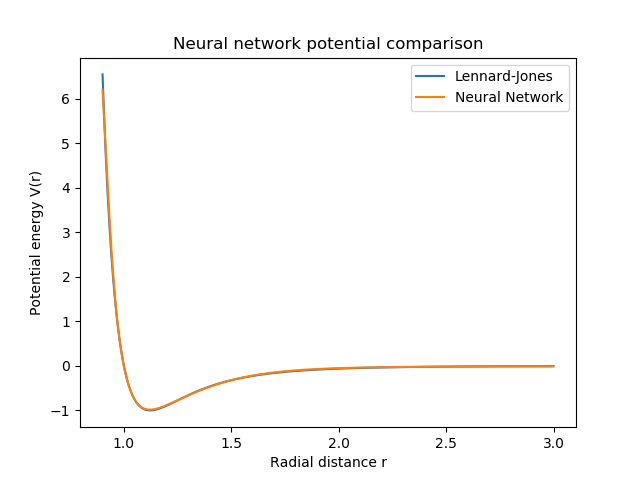
\includegraphics[width=\linewidth]{potential_comparison.png}
    \caption{Neural network potential compared to Lennard-Jones.}
    \label{fig:potential-comparison}
\end{figure}

\begin{figure}[h]
    \centering
    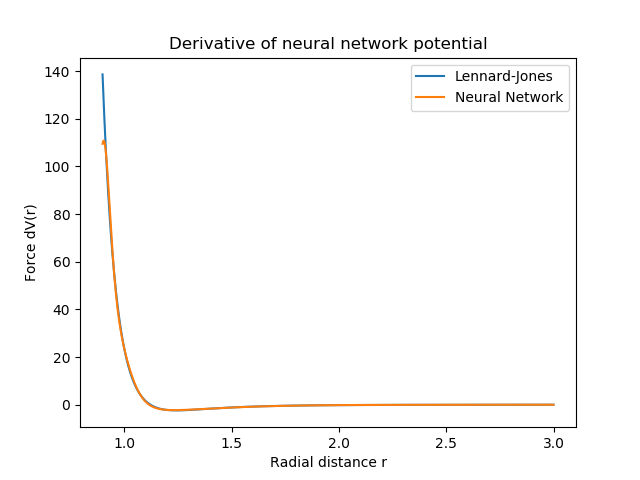
\includegraphics[width=\linewidth]{force_comparison.png}
    \caption{Neural network derivative compared to Lennard-Jones.}
    \label{fig:force-comparison}
\end{figure}

\begin{figure}[h]
    \centering
    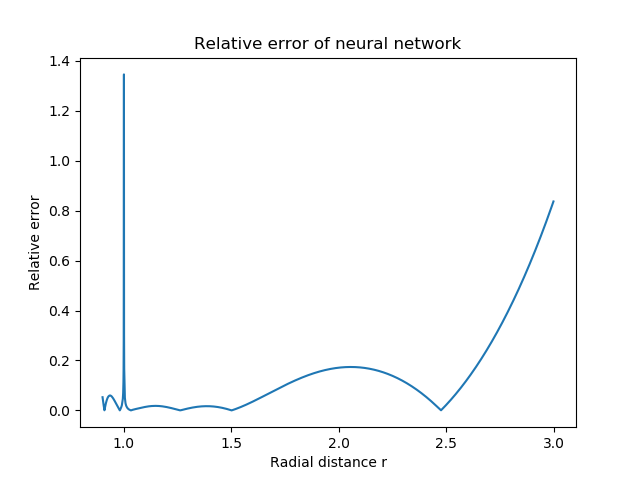
\includegraphics[width=\linewidth]{potential_relative_error.png}
    \caption{Relative error of the neural network potential compared
        to Lennard-Jones.}
    \label{fig:potential-rel-error}
\end{figure}

\begin{figure}[h]
    \centering
    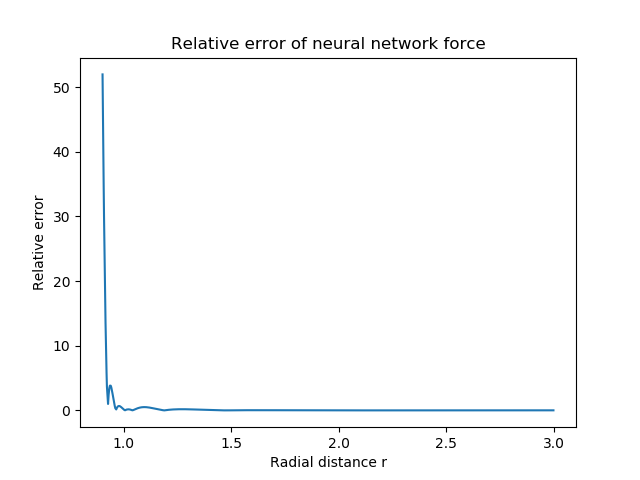
\includegraphics[width=\linewidth]{force_relative_error.png}
    \caption{Relative error of neural network derivative compared
        to Lennard-Jones.}
    \label{fig:force-rel-error}
\end{figure}
